\documentclass[letterpaper, 10 pt, conference]{ieeeconf}  

\IEEEoverridecommandlockouts                             
\overrideIEEEmargins

\usepackage{graphics} 
\usepackage{graphicx}
\usepackage{epsfig} 
\usepackage{mathptmx} 
\usepackage{times} 
\usepackage{amsmath} 
\usepackage{amssymb}  
\usepackage{makeidx}
\usepackage{float}
\usepackage{balance}
\usepackage{url}
\usepackage[hidelinks]{hyperref}
\usepackage{cite}
\usepackage{flexisym}
\usepackage{chngcntr}
\usepackage{amsmath}
{
%      \theoremstyle{plain}
      \newtheorem{assumption}{\textbf{Assumption}}
      \newtheorem{definition}{\textbf{Definition}}
      \newtheorem{proposition}{\textbf{Proposition}}
      \newtheorem{lemma}{\textbf{Lemma}}
      \newtheorem{theorem}{\textbf{Theorem}}
}
\DeclareMathOperator*{\maxi}{max}
\DeclareMathOperator*{\mini}{min}

%----------------------------------------------

\title{\LARGE \bf Cooperative Mobile Manipulation with Implicit Communication}

\author{George P. Kontoudis
\thanks{This work was submitted on 02/05/17 and is part of the project for the class AOE5984-Cyber-Physical Systems \& Distributed Control, offered by Prof. Kyriakos Vamvoudakis, \url{kyriakos@vt.edu}}
\thanks{G. Kontoudis is with the Mechanical Engineering Department, Virginia Polytechnic Institute and State University, Blacksburg, VA, 24060, USA, \url{gpkont@vt.edu}}}

\begin{document}
\maketitle
\thispagestyle{empty}
\pagestyle{empty}

%----------------------------------------------

\begin{abstract}
A solution for the cooperative mobile manipulation problem of a group of N robots is presented. The main contribution of this methodology lies in the utilization of local information for robot coordination, without explicit communication. Local information for motion coordination is achieved through force feedback. The object's translational and rotational motion can be efficiently controlled. The proposed methodology can alter the leader either with a robot or with a human. The efficacy of the proposed method is verified through simulations, considering force analysis of agents.   
\end{abstract}

\normalsize{\bf\small\emph{Index Terms:} mobile manipulation, cooperative control, consensus algorithms}  

%----------------------------------------------

\section{Introduction}\label{intro}

A multi-robot manipulation algorithm which integrates local information is presented \cite{wang2016force}. Multi-robot cooperation can be accomplished without explicit communication, but only with local information. The suggested local information is force feedback, gathered and processed individually from each robot. The leader can be either a robot or a human, but in each case operates as the dominant agent of motion planning. The desired trajectory is imposed by the leader while the followers regulate their forces according to the leader's amplitude and direction.   

Multi-agent networks with communication face several problems. Communication is usually very noisy, demands high computational power, deals with uncertainty and in some cases might get vanished. The relationship of the number of nodes with communication complexity is proportional, that means for large networks a major issue lies in communication between agents. An interesting approach is to neglect communication between agents and design a strategy to attain consensus through force feedback for each agent locally. In this way, communication problems can be fully confronted, so update of the network can be managed at any time. 

Robotic manipulation is an emerging field for many decades. In case we consider each robot as a finger, and each local attachment point as a contact point, then we get similar structure and properties with multi-fingered grasping and manipulation tasks \cite{murray1994mathematical}, \cite{prattichizzo2016grasping}. However, after efficiently grasp an object with several robots, we need to maintain a stable grasp by applying effective caging strategies \cite{fink2008multi}, \cite{pereira2004decentralized}. Transferring objects with multiple robots demands an untrivial motion planning approach \cite{donald1997information}, \cite{rus1995moving}. Multi-agent consensus is a similar field, which is employed to develop force consensus between agents without communication \cite{jadbabaie2003coordination}, \cite{olfati2007consensus}, \cite{ren2005consensus}. The whole procedure is bio-inspired from ant colonies, as it recognized that ants have a specific leader when they cooperate to move objects \cite{gelblum2015ant}. Moreover, ants do not explicitly communicate, but instead they employ object's vibration and/or deformation to coordinate their motion \cite{mccreery2014cooperative}. 

In this project we implement 2D planar motion of robots and object $Q \in \mathbb{R}^2$. We consider $N$ robots of a set $R_i$, with $i=1, \hdots ,N$, where $R_1$ is always the leader, and the other robots are the followers. Therefore, the leader drives the system by following a desired trajectory, that is unknown to the rest robots. Moreover, any form of communication is forbidden along agents. The motion control algorithm using force feedback consists of two steps. First, the followers need to recognize the leader's force magnitude and direction, by employing force feedback. Then, the followers have to cooperate and provoke a resultant force in the same direction and with larger amplitude.  Furthermore, two different force analyses were occurred as object shape and mass may be varied. In the first case, an analysis of drugging low-weight objects is presented, while in the second case an analysis for heavy-weight objects, which assumed to be placed on a moving platform, is provided. 

Difficulties that we expect to face are to determine whether this technique is accurate and robust in terms of following the desirable trajectory of the leader and not damage the object. Then, the performance of the proposed technique should exceed the performance of cooperative multi-robot systems with explicit communication. Simulation of the problem is ideal to be implemented, but it also accounts of avoiding collision for every agent. Therefore, we study a cooperative mobile manipulation technique without communication, by simulating the force magnitude and tracking the direction of the leader from the follower agents.

The remainder of this report is organized as follows. Section \ref{pf} discusses the problem formulation. The efficacy of the proposed methodology is assessed in Section \ref{sim} by a set of simulations. Finally, Section \ref{concl} provides the conclusions of the studied methodology and gives directions for future work.

%----------------------------------------------

\section{Problem Formaulation}\label{pf}
In this section we formulate the proposed methodology for planar cooperative manipulation without communication, using force feedback. We study 2 different force feedback cases. First, we deal with the manipulation of lightweight objects that can be efficiently moved from a small number of robots. This methodology studied in   \cite{wang2016force}, \cite{wang2016kinematic} and characterized as constant boost force (CB-ANTS). Next, we analyze the condition of heavyweight objects where the robots lift and carry the object for its motion in 2-$D$ space as in \cite{wang2015multi}, \cite{wang2016force}, where this method refered as proportional force (P-ANTS). The reason that the two methodologies were discriminate is keen on friction. The friction for the motion of rigid bodies is divided in two terms, the static and the kinetic. Static friction is proportional to the applied force and dominates while the rigid body is not moving. The maximum value of static friction coefficient emerges just before slipping. In case that the applied forces overcome the static friction the motion of the object appears. While the object is sliding the only friction that applies is the kinetic. In most cases the coefficient of static friction is greater than the coefficient of kinetic friction \cite{tipler2007physics}. If the object is lightweight we can easily produce drag forces to overcome the static friction, but when the object is heavyweight the problem becomes nontrivial. Therefore the methodology suggests for heavyweight objects to lift and drag it by robots. In such case, the kinetic friction becomes negligible and the coefficient of static friction of the rollers is significantly lower than the coefficient of kinetic friction while the object is sliding on the ground. Furthermore, we do not have to deal with the static friction of the object. Depending on the weight, similar techniques are followed by humans to relocate objects. 

\subsection{Rigid Body Dynamics}\label{rbd}
In this section we study the object as rigid body and the relevant dynamics are presented. Given the object's mass $M$ in ($kg$), and acceleration of gravity $g$ in $m/s^2$. The applied forces of the robots are indicated as $\{ F_1, F_2, \hdots, F_N \}$ in $N$, and the linear velocity of the object as $v$ in $m/s$. We assume that the coefficient of kinetic friction $\mu_k$ is constant and its direction is always opposed to the object's velocity vector. Moreover, the coefficient of static friction $\mu_v$ is proportional to the object's applied force. The translational motion of the object is subject to the second law of Newton. The object's dynamics for translational movement can be described as 
\begin{equation}
M\dot{v}=\sum_{i=1}^N F_i-\mu_{k}Mg\frac{v}{||v||}-\mu_v v.
\end{equation}

In case we drag the object (F-ANTS) we can eliminate the static friction because we assume that the object is moving, and thus we discretize by employing Euler's method 
\begin{equation}\label{dod}
M\frac{v_{t+1}-v_t}{\Delta t}=\sum_{i=1}^N F_i(t)-\mu_kMg\frac{v_t}{||v_t||}.
\end{equation}
For heavyweight objects we only consider the static friction of the rollers, which yields 
\begin{equation}
M\dot{v}=\sum_{i=1}^N F_i-\mu_v v.
\end{equation}

In this study we assume that the object's mass, the coefficient of kinetic friction, the coefficient of static friction, the acceleration of gravity, and the number of robots, that take part to the cooperative manipulation of the object, are given for all robots.
\begin{assumption}\label{as1}
\textit{All robots have information about the exact values of $M$, $\mu_k$, $\mu_v$, $g$, $N$.}
\end{assumption}
 
\subsection{Rotational Dynamics}\label{rd}
In this section the rotational dynamics of the object and the local measurement, that the robots can gather about the object's motion, are discussed. Measurement of the object's velocity in center of mass (CoM) is not feasible to be taken in practice. However we can get information from the robot about the translational velocity and the angular velocity at the contact point. \vspace{.2cm}
\begin{assumption}\label{as2}
\textit{The leader have information about the angular velocity of the object and applies a torque $T_1$.} \vspace{.2cm}
\end{assumption}
Given the object's moment of inertia $J$ in $kg-m^2$, the angular velocity $\omega$ in $rad/s$, and under the Assumption \ref{as2} we can derive the overall rotational dynamics of the studied object as follows
\begin{equation}\label{rotDyn1}
J\dot{\omega}=T_1 +\sum_{i=2}^{N}r_i\times F_i-T_f,
\end{equation}
where $T_f$ is the torque related with the static friction, $\sum_{i=2}^{N}r_i\times F_i$ is the torque produced by the follower robots, $r_i$ is the vector from the object's center of mass to the contact point of the $i$-robot,  and $T_l$ is the torque imposed by the leader robot.\vspace{.2cm}
\begin{proposition}\label{pr1}
\textit{For any rigid body object with an arbitrary shape in a planar region $Q \in \mathbb{R}^2$ the frictional torque caused by the static friction is given as}
\begin{equation}
T_f=-\frac{\mu_{\nu}}{M}J\omega.
\end{equation} \vspace{.2cm}
\end{proposition}
As a result the overall rotational dynamics of equation \ref{rotDyn1} under Porposition \ref{pr1} yields
\begin{equation}
J\dot{\omega}=T_1 +\sum_{i=2}^{N}r_i\times F_i--\frac{\mu_{\nu}}{M}J\omega.
\end{equation}\label{rotDyn2}

Since we study object's as rigid bodies the only feasible contact points for the robots to grasp the object are at the object's perimeter. Furthermore, if the mass of the rigid body is not evenly distributed it becomes difficult to get the exact position of the object's center of mass. The information that we can get are the measurements of contact points and the translational velocity of the object. The local motion measurements include the velocity and the acceleration of the robot at the contact point, that can be written in global reference of the object's center of mass 
\begin{equation}
v_i=v_c +\omega \times r_i,
\end{equation}
\begin{equation}
\dot{v}_i=\dot{v}_c +\dot{\omega }\times r_i+\omega \times (\omega \times r_i),
\end{equation}
where $v_i,$, $\dot{v_i}$ are the velocity and the acceleration at the contact point respectively. Since, that contact points to the object are fixed, Coriolis acceleration does not exist. An important issue that arises with the object's rotation is that the each robot has a different motion measurement, that prevents for effective analysis. Thus, the local measurement study is not reproduced with simulations in this project. In case that we did not have time restrictions we could perform experiments with real robots and gather data to validate the efficacy of the suggested methodology.

An important aspect for the efficiency of the proposed methodology deals with the position of the contact points. To guarantee the performance of the proposed methodology Assumption \ref{as3} should be made.\vspace{.2cm}
\begin{assumption}\label{as3}
\textit{The contact points are centrosymmetric with respect to the object's center of mass, so $\sum_{i-1}^{N}r_i=0$.} \vspace{.2cm}
\end{assumption}
Under Assumption \ref{as3} and if the forces of all robots converge to a value the second term of equation \ref{rotDyn2} is vanished. In practice centrosymmetry assumption is difficult to be achieved, because we do not have knowledge about the exact center of mass for the studied objects.

\subsection{Constant Boost Force (CB-ANTS)}\label{cb}
In this section we present the constant boost force (CB-ANTS) case, where the robots drag the object through the desired trajectory to the goal position. Kinetic friction is the dominant friction and we assume that the coefficient of kinetic friction has a constant value. First, the methodology is based on the global information of the object's velocity at the center mass. Next, the exploitation of only local information at the contact points of each robots is employed to study a force feedback controller.

The follower's force feedback controller is designed as follows
\begin{equation}\label{cbfc}
F_i^c=\frac{\mu_k Mg}{N}\frac{v^c}{||v^c||}, \hspace{.2cm} i=\{ 2,3,\hdots , N\},
\end{equation}
where $i$ are the follower robots, $v^c$ is the velocity of the object at the center of mass, and $\hat{v}^c=\frac{v^c}{||v^c||}$ is the unit tangent vector that gives us the direction of the force. This force feedback controller was selected because it combines the velocity of the object at the center of mass which provide information for the leader's motion intention. Moreover, the restriction of follower's forces result the dominance  of the leader's force.

The leader's force feedback controller is designed as follows
\begin{equation}\label{cblc}
F_l^l= f_d \frac{v_d^l}{||v_d^l||}= K_pmax\{ ||v_d^l||-||v^l||,0 \}\frac{v_d^l}{||v_d^l||},
\end{equation}
where $v_d^l$, $v^l$ is the desired and the current velocity of the leader robot respectively, $K_p$ is the proportional gain, and $\hat{v}_d=\frac{v_d^l}{||v_d^l||}$ is the unit tangent vector of the desired force of the leader robot. The max function is utilized to track the leader's velocity and switch to $0$ when it reached in order to maintain the correct direction. The overall goal of the leader robot force feedback controller is to steer the object through a specific trajectory to the goal position.

We rely on Lemma \ref{lem1} to achieve consensus. \vspace{.2cm}
\begin{lemma}\label{lem1}
\textit{Given a discrete system $v_t$ is calculated as follows
\begin{equation}
v_{t+1}=\alpha_1 w+\beta_1 v_t,
\end{equation}
where $w$ is a vector with constants, $\{ \alpha_t|\alpha_t \geq 0, a_0^2+a_1^2+\hdots +a_t^2 \neq 0 \}$, and $\{ \beta_t|0<\beta_t<1 \}$. Then, $v_t$ converges to the direction of $w$ as $t \rightarrow \infty$ with a constant rate
\begin{equation}
v_t \rightarrow \gamma w,
\end{equation}
where $\gamma >0$ and has the form of
\begin{equation}
\gamma =\alpha_{t-1} + \beta_{t-1}\alpha_{t-2}+\beta_{t-2}\beta_{t-1}\alpha_{t-3}+\hdots+\beta_{t-1}\hdots \beta_1\beta_0\alpha_0.
\end{equation}} \vspace{.2cm}
\end{lemma}
\begin{theorem}\label{thrm1}
\textit{In the constant boost force (CB-ANTS) case by employing equations \ref{dod}, \ref{cbfc}, \ref{cblc} all follower robots align to the leader's direction and converge at a boost consensus value 
\begin{equation}
\phi = (N-1)\frac{\mu_kMg}{N},
\end{equation}
with time step $0<\Delta t<N\frac{||v_t||}{\mu_kg}$. Moreover object's velocity converge to the leader's desired velocity.} \vspace{.2cm}
\end{theorem}
The dynamic equations that we utilize for the constant boost force (CB-ANTS) case are expressed as
\begin{equation}
v_{t+1}= \Bigg(1-\frac{\mu_k g \Delta t}{N||v_t||}\Bigg)v_t+ \frac{\Delta t K_pmax\{ ||v_d^l||-||v^l||,0 \}}{M ||v_d||}v_d
\end{equation}
Note that the leader robot has to have specific force abilities to steer the object. That reveals the leader robot's demanding force, which needs to be at least above the value $\mu_kMg/N$. 

Since the convergence is guaranteed, the study of the convergence rate is mandatory to evaluate the performance of the methodology.
\begin{theorem}\label{thrm2}
\textit{The converge of follower's forces to the leader's force is succeeded with an exponential fast rate.} \vspace{.2cm}
\end{theorem}

\subsection{CB-ANTS using Local Measurements}\label{cblm}
In this section the analysis of
Follower's controller with local measurement
\begin{equation}
F_i=\frac{\mu_kMg}{N}\frac{v_t+\omega_t\times r_i}{||v_t+\omega_t\times r_i||}
\end{equation}
Object's Dynamics with local measurements
\begin{equation*}
v_{t+1}= \frac{\Delta t}{M}f_d\frac{v_d}{||v_d||}+\sum_{i=2}^N \bigg(\frac{\mu_k g \Delta t}{N||v_t+\omega_t \times r_i||} \bigg) \omega_t \times r_i+
\end{equation*}
\begin{equation}
+\Bigg(1+\sum_{i=2}^N \frac{\mu_k g \Delta t}{N||v_t + \omega_t \times r_i||}-\frac{\mu_k g \Delta t}{||v_t||}\Bigg)v_t
\end{equation}
\begin{equation}
||\omega_t||<\frac{||v_t||}{N||r_m||}
\end{equation}
$m=\max\limits_{i}||r_i||$, $i=2,\hdots,N$
\begin{equation}
\Bigg| \Bigg| \sum_{i=2}^N \Bigg( \frac{\mu_k g \Delta t}{n||v_t+ \omega_t \times r_i||} \Bigg)\omega_t \times r_i \Bigg| \Bigg|< \frac{\mu_k g \Delta t}{N} \Bigg( \frac{2N-1}{N^2-N} \Bigg)
\end{equation}
$(2N-1)/(N^2-N)$
%----------------------------------------------

\section{Simulations}\label{sim}
\begin{figure}[!h]
	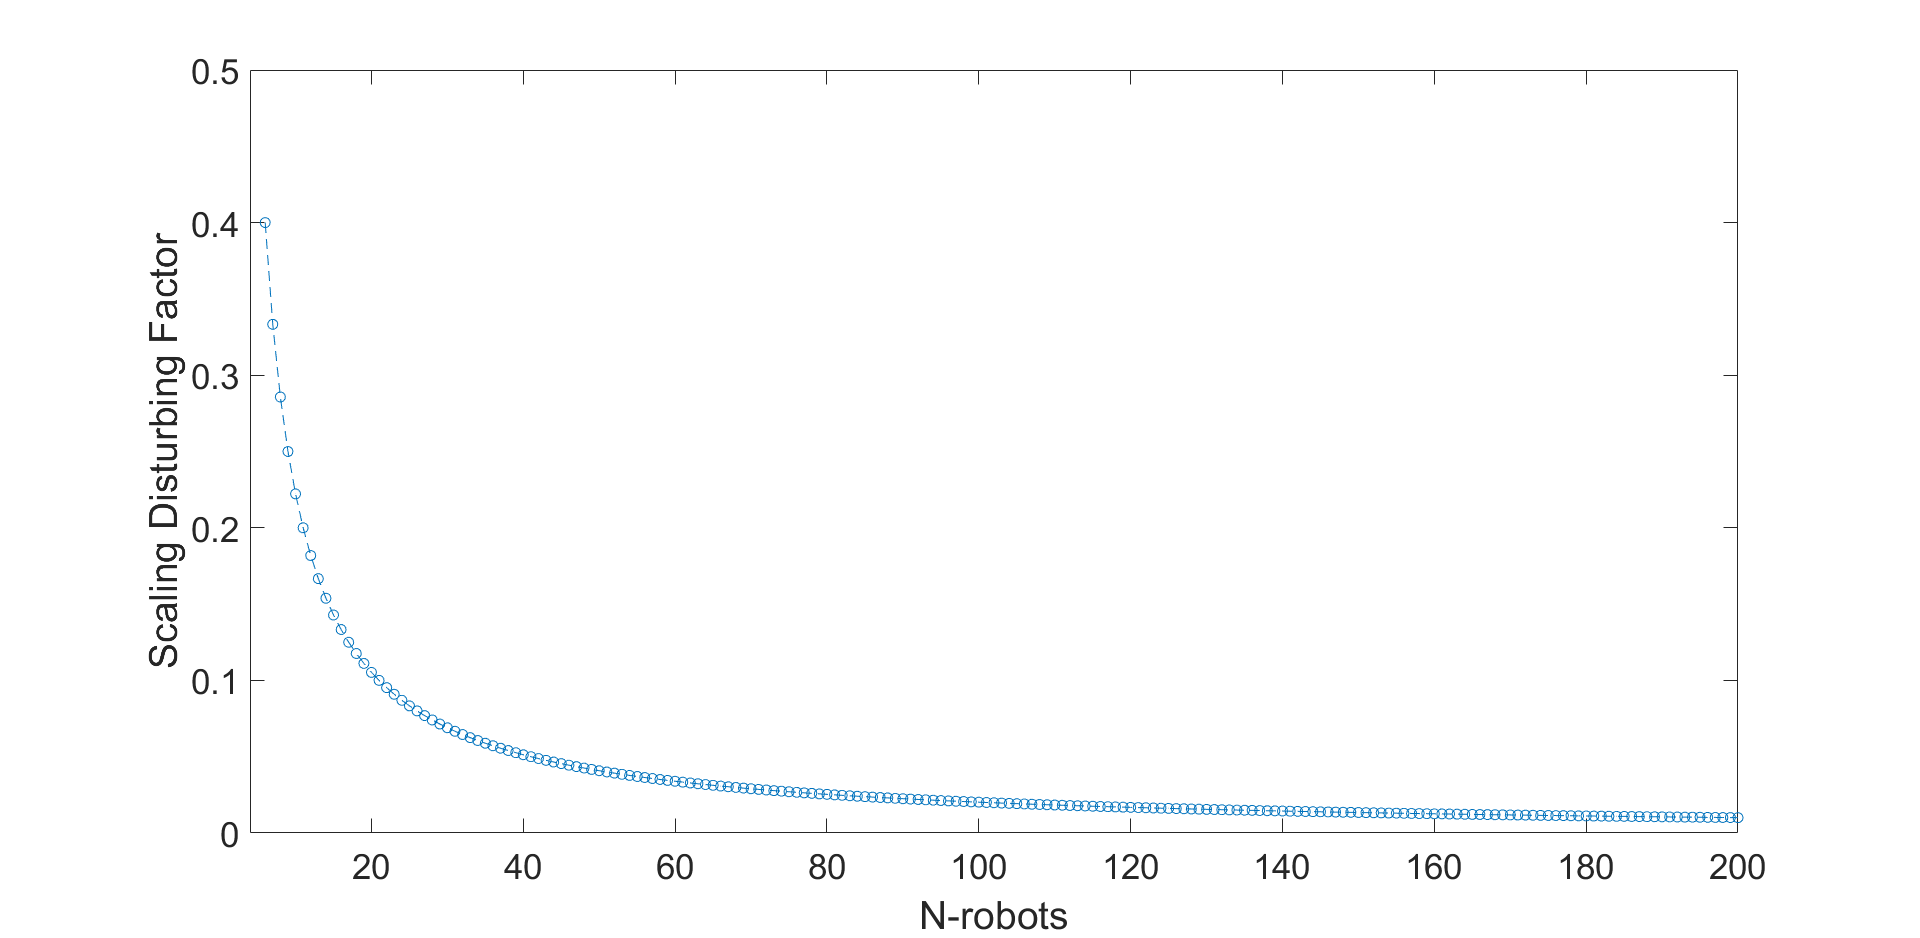
\includegraphics[width=.53\textwidth]{figures/scalingFactorDisturbance.png}
	\centering
	\caption{Scaling down of disturbing factor.}
	\label{scaling}
\end{figure}
\begin{figure}[!h]
	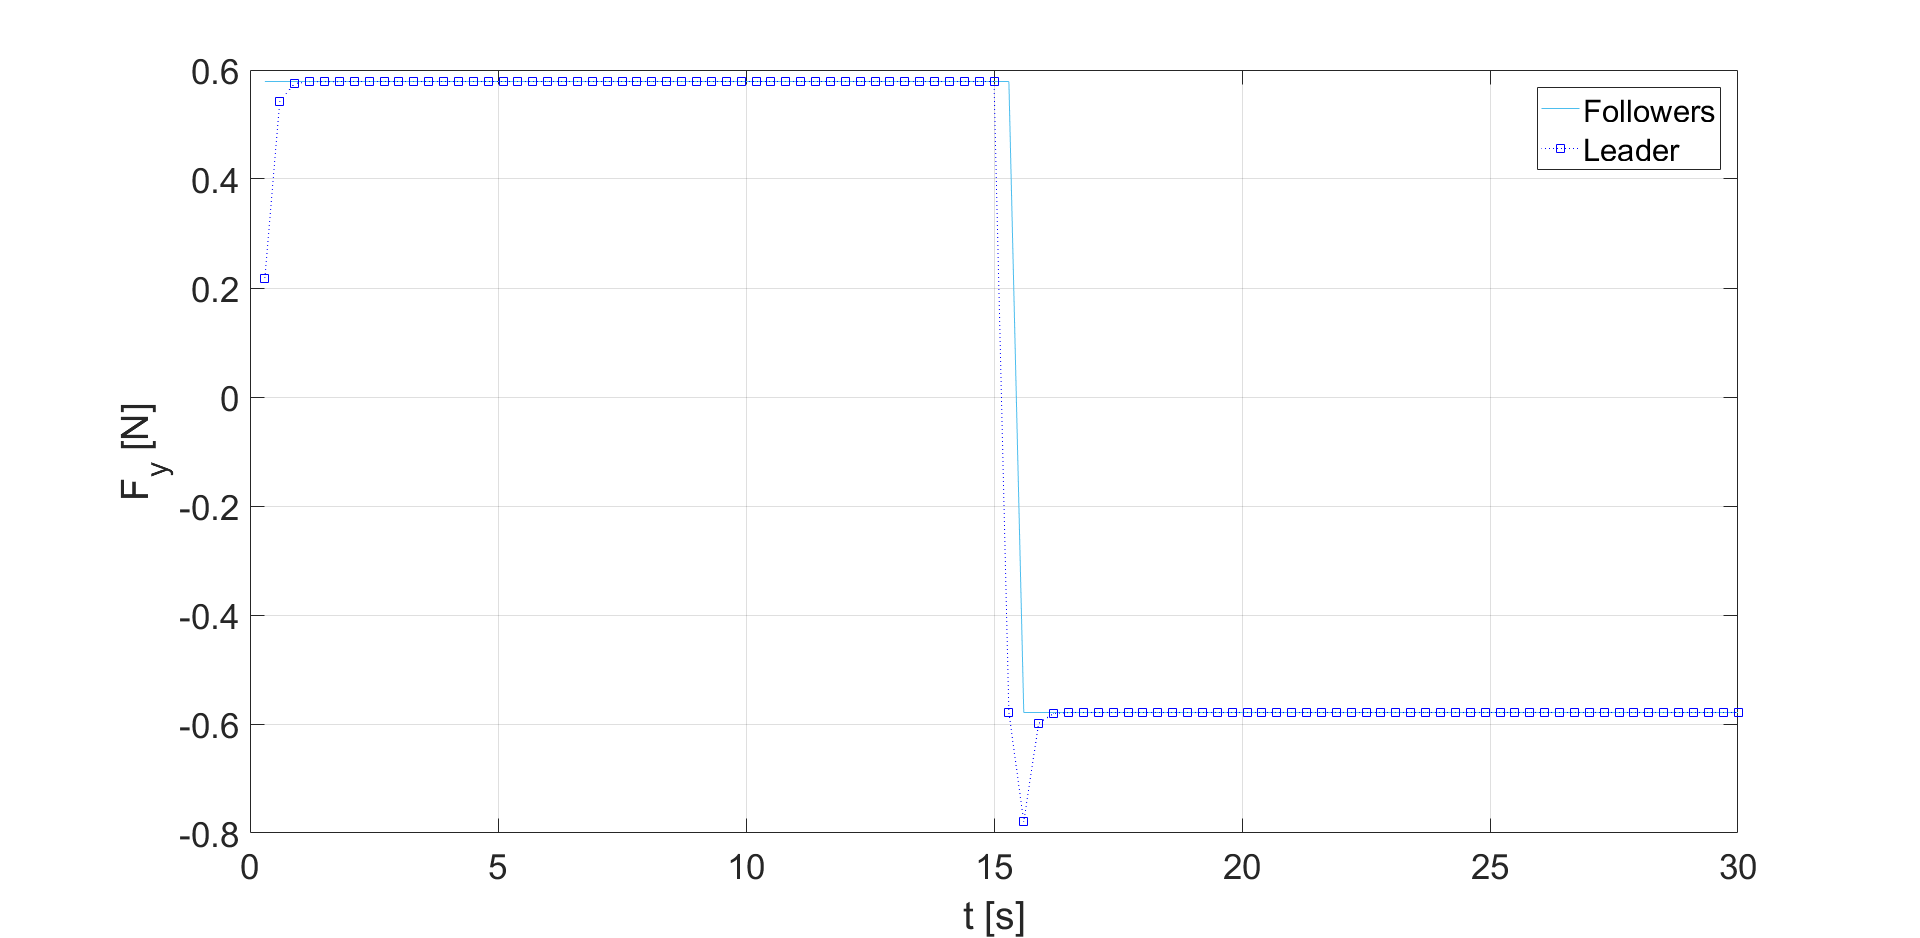
\includegraphics[width=.53\textwidth]{figures/CB_ANTS_Fy.png}
	\centering
	\caption{CB-ANTS $F_y$.}
	\label{fcbfy}
\end{figure}
\begin{figure}[!h]
	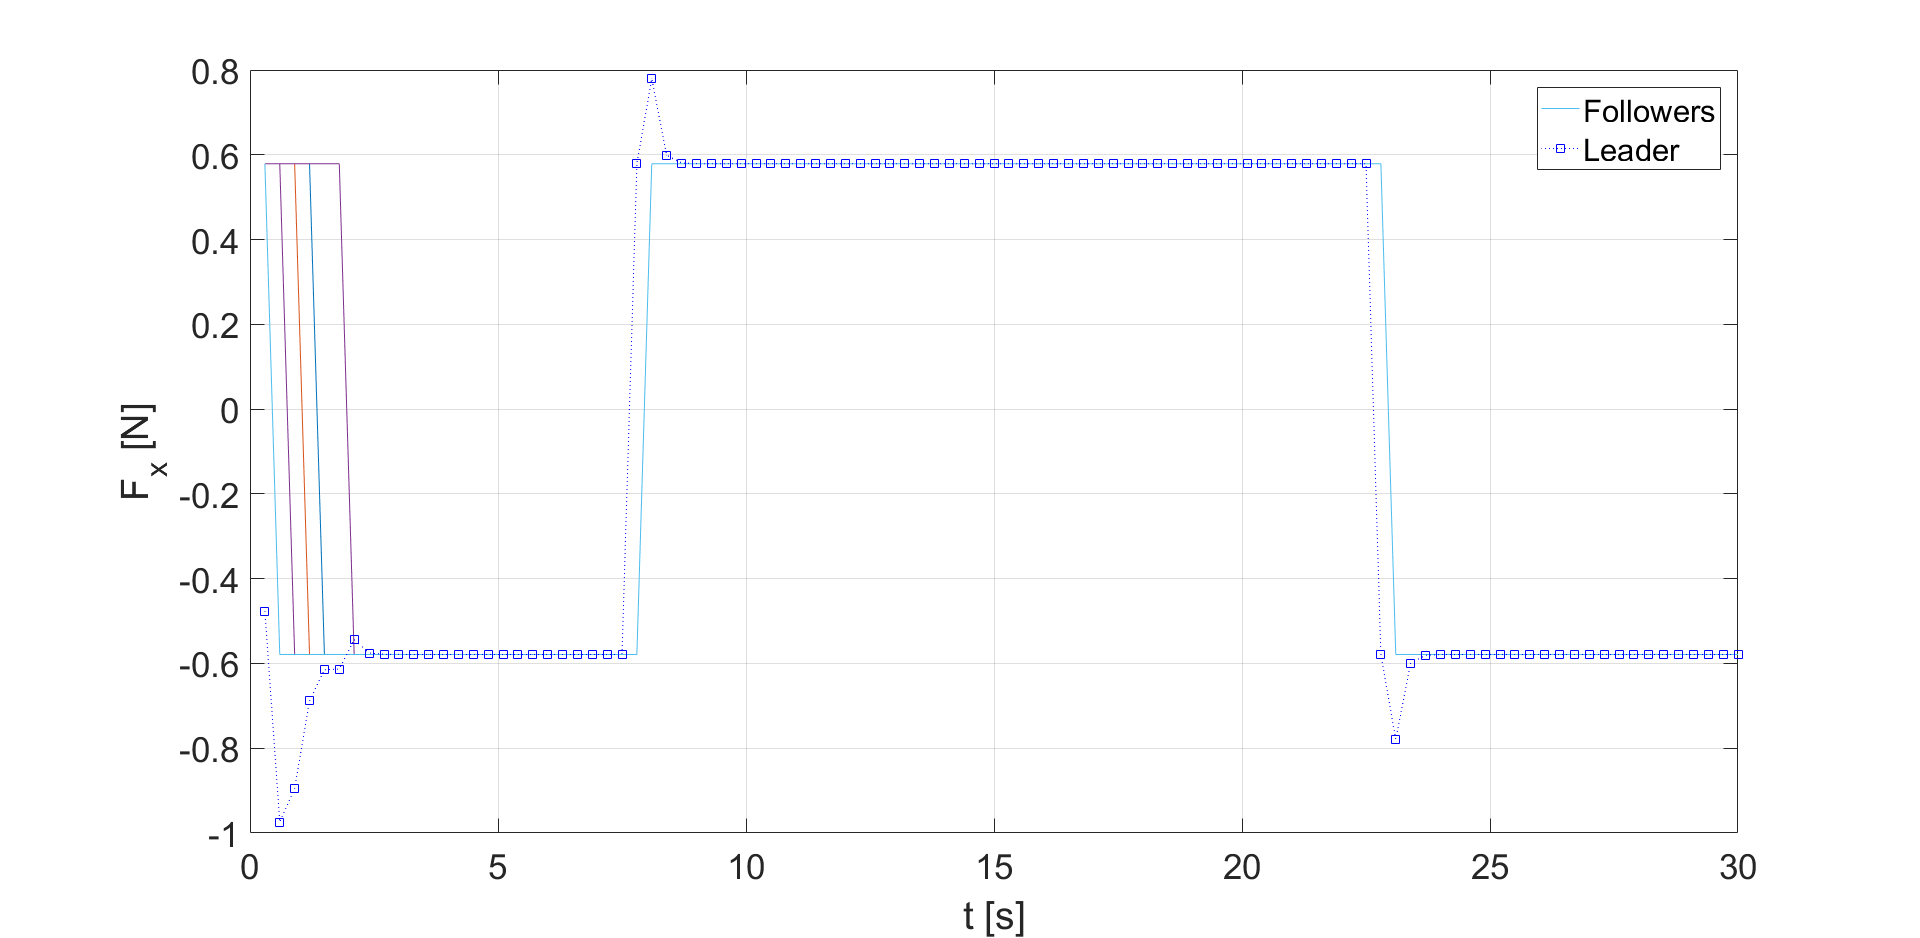
\includegraphics[width=.53\textwidth]{figures/CB_ANTS_Fx.png}
	\centering
	\caption{CB-ANTS $F_x$.}
	\label{fcbfx}
\end{figure}
\begin{figure}[!h]
	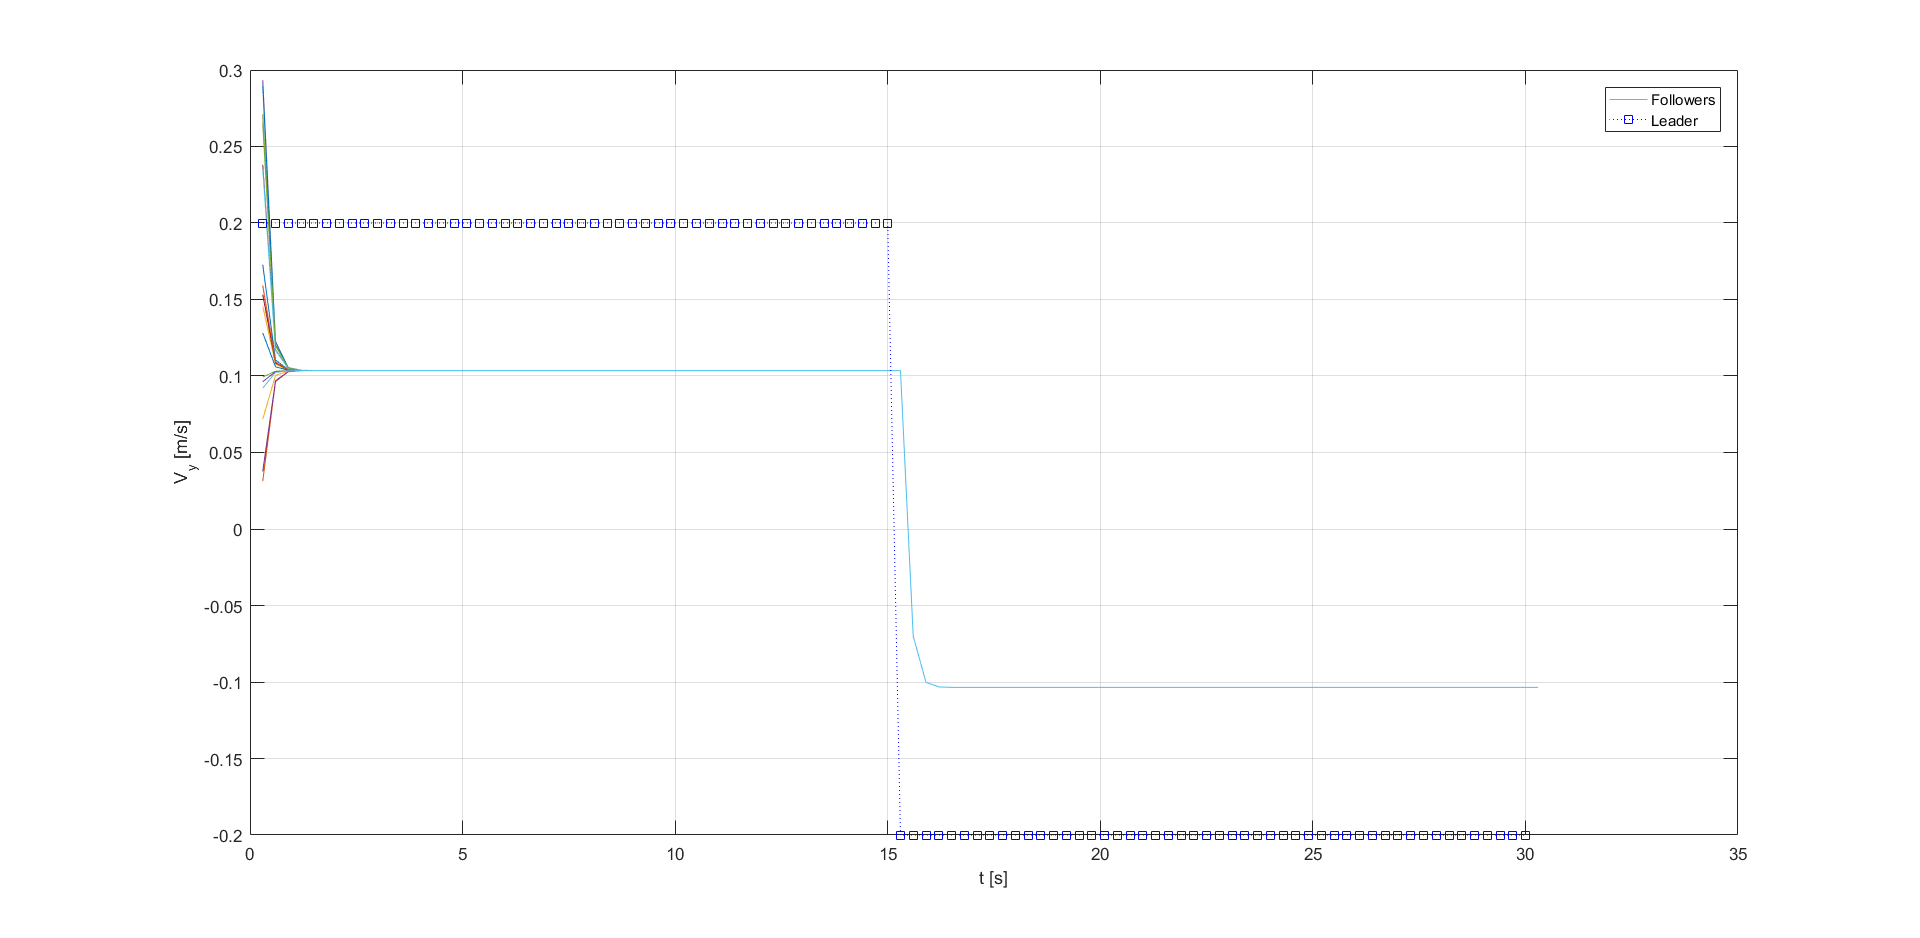
\includegraphics[width=.53\textwidth]{figures/CB_ANTS_Vy.png}
	\centering
	\caption{CB-ANTS $V_y$.}
	\label{fcbvy}
\end{figure}
\begin{figure}[!h]
	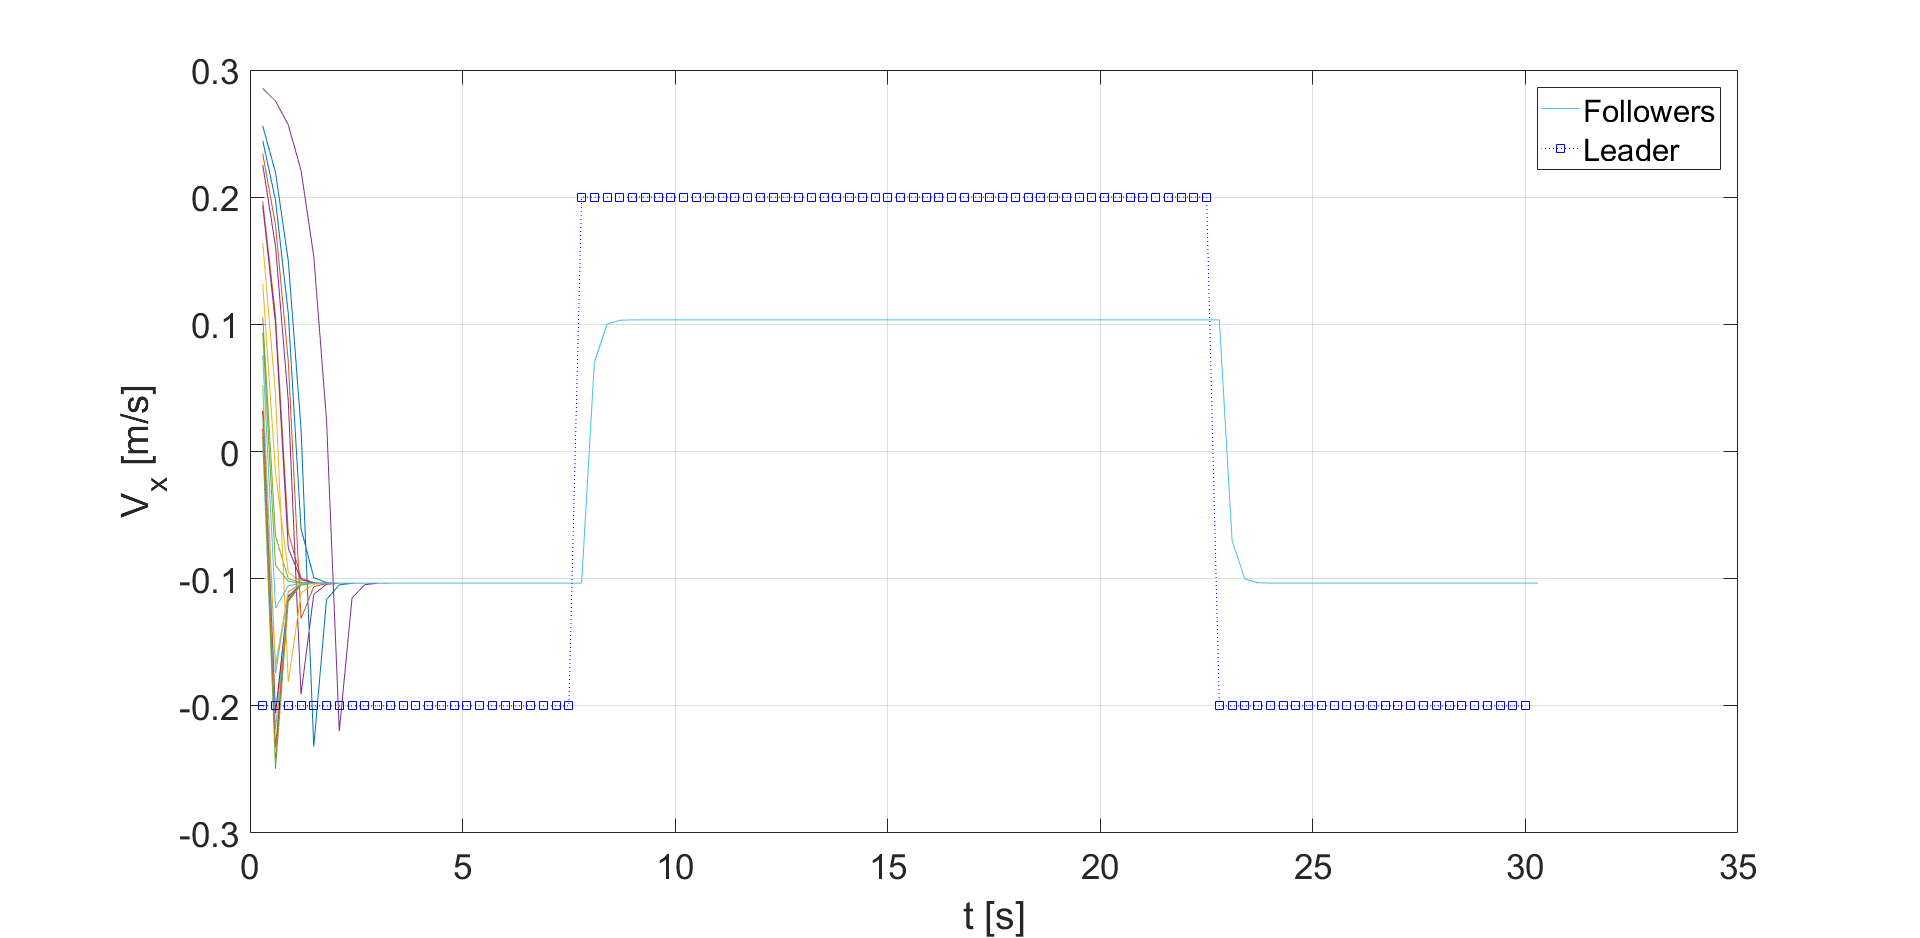
\includegraphics[width=.53\textwidth]{figures/CB_ANTS_Vx.png}
	\centering
	\caption{CB-ANTS $V_x$.}
	\label{fcbvx}
\end{figure}

\begin{figure}[!h]
	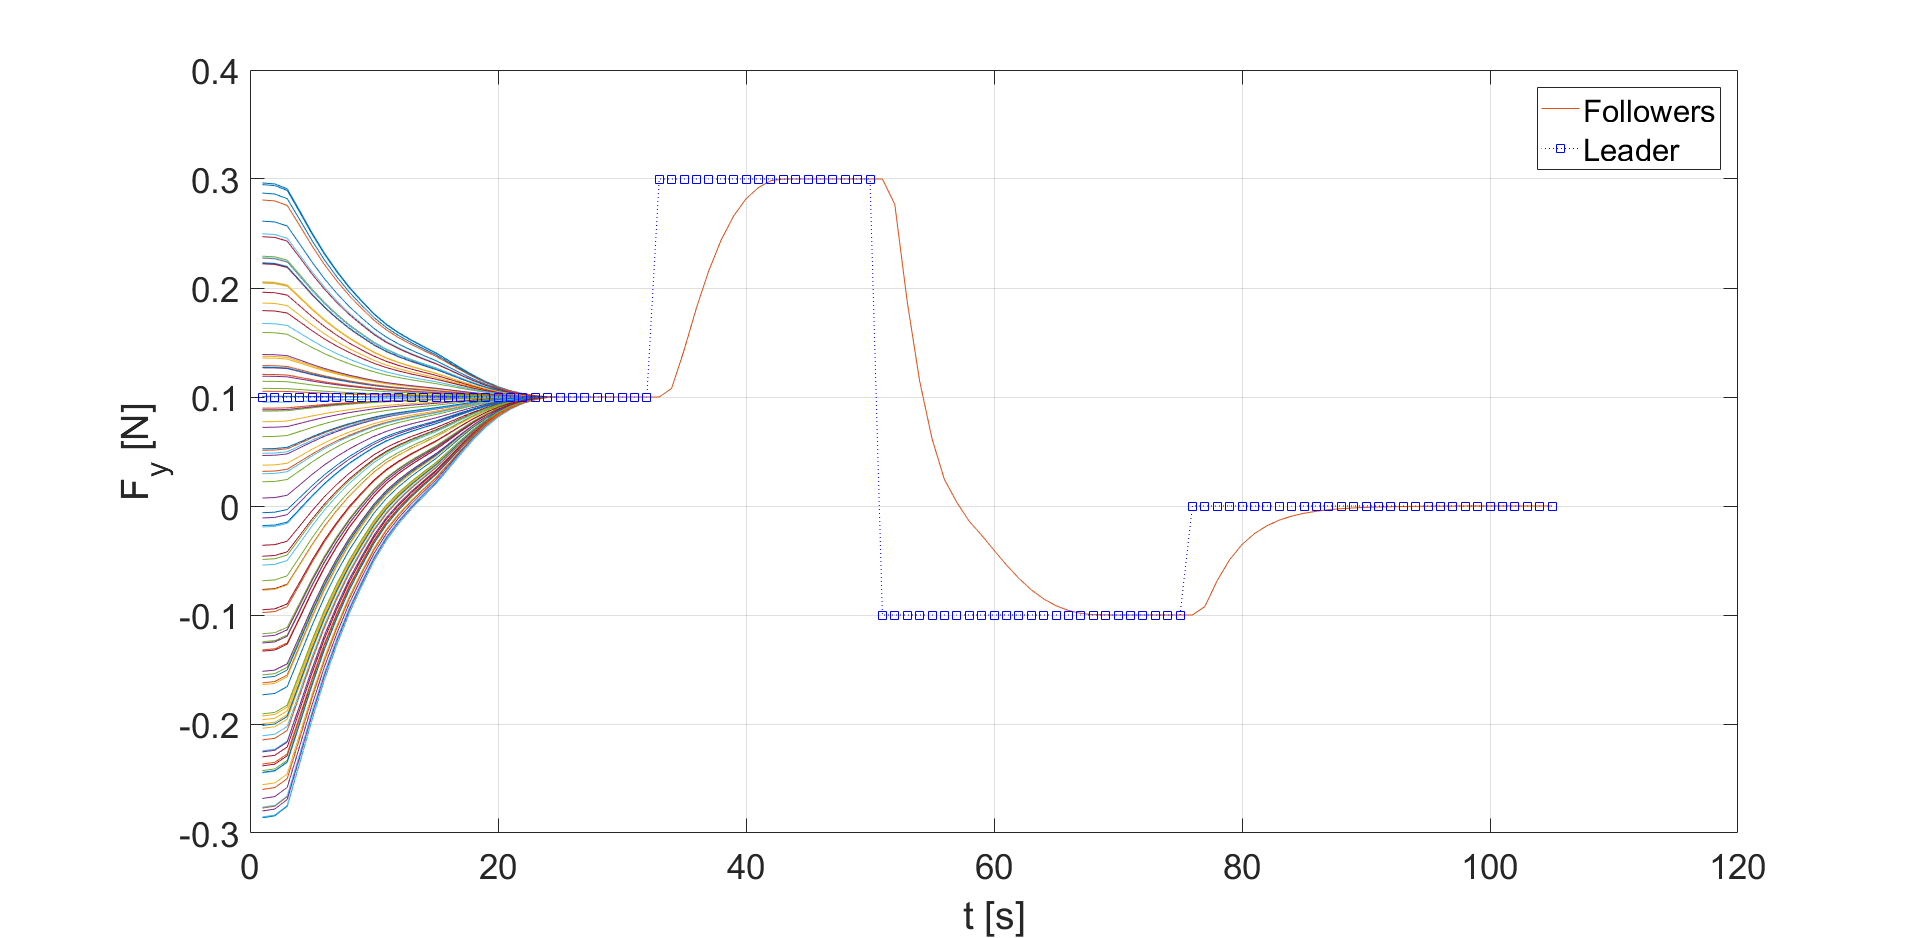
\includegraphics[width=.53\textwidth]{figures/P_ANTS_Fy.png}
	\centering
	\caption{P-ANTS $F_y$.}
	\label{fpfy}
\end{figure}
\begin{figure}[!h]
	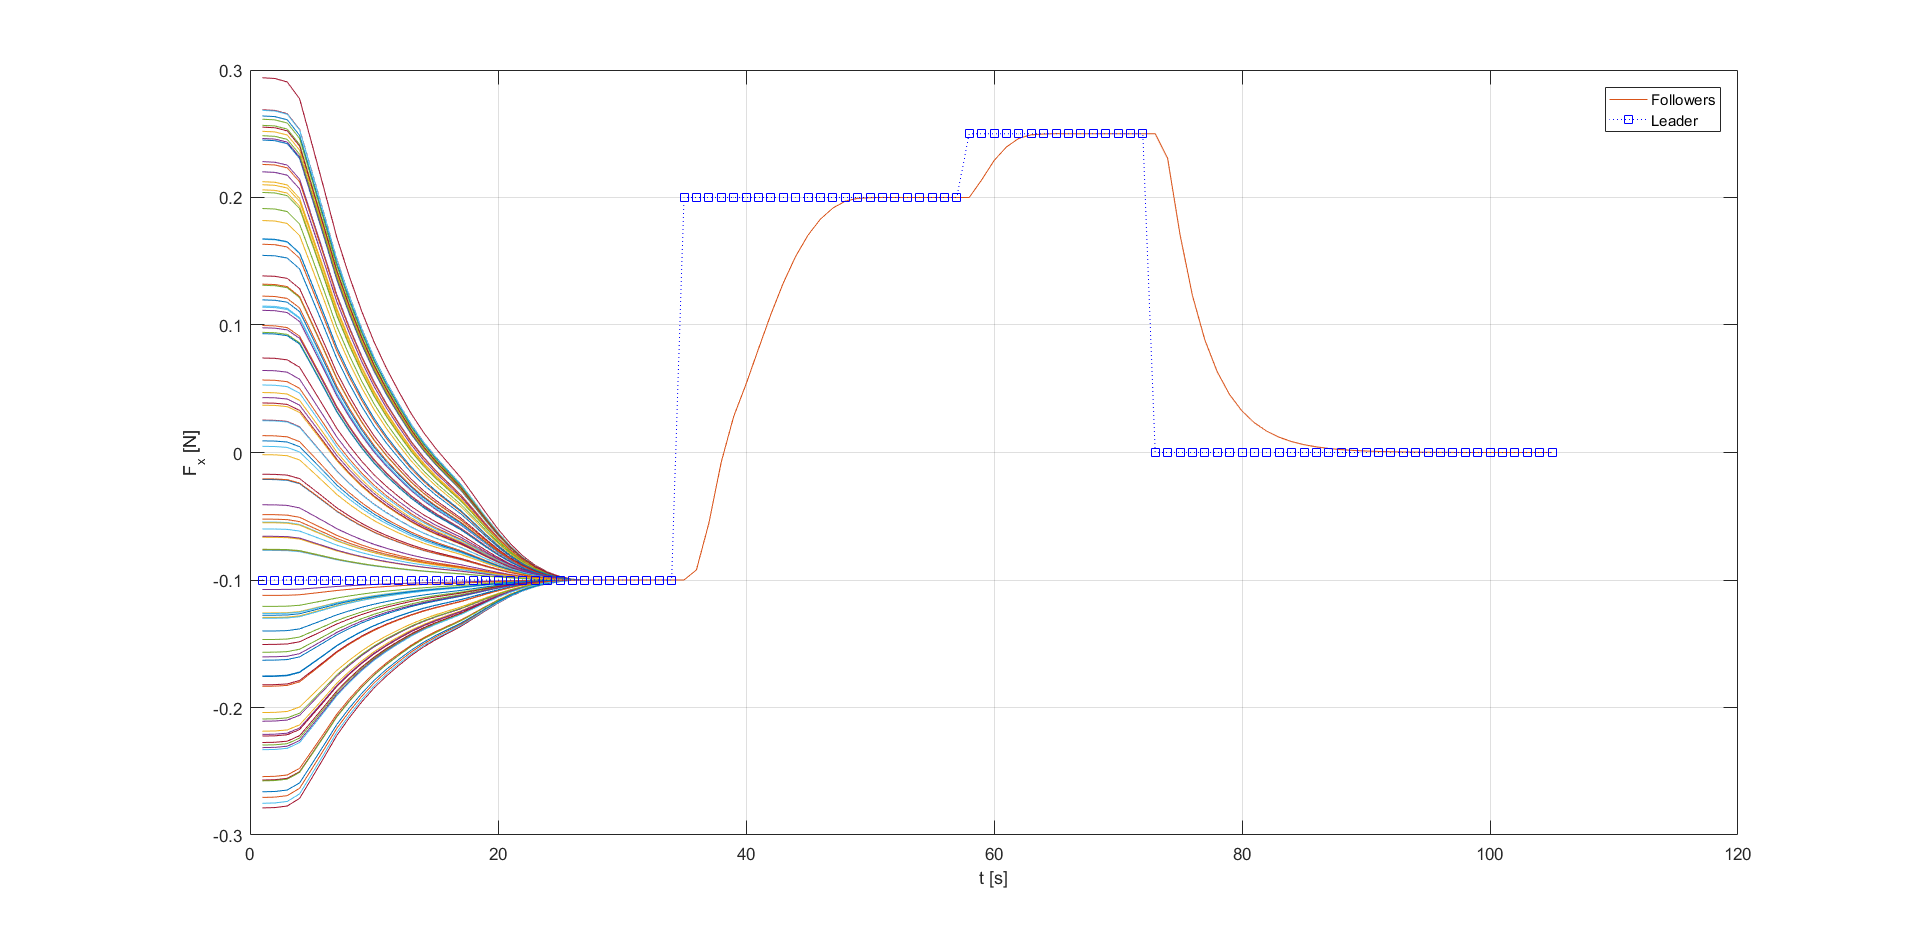
\includegraphics[width=.53\textwidth]{figures/P_ANTS_Fx.png}
	\centering
	\caption{P-ANTS $F_x$.}
	\label{fpfx}
\end{figure}
\begin{figure}[!h]
	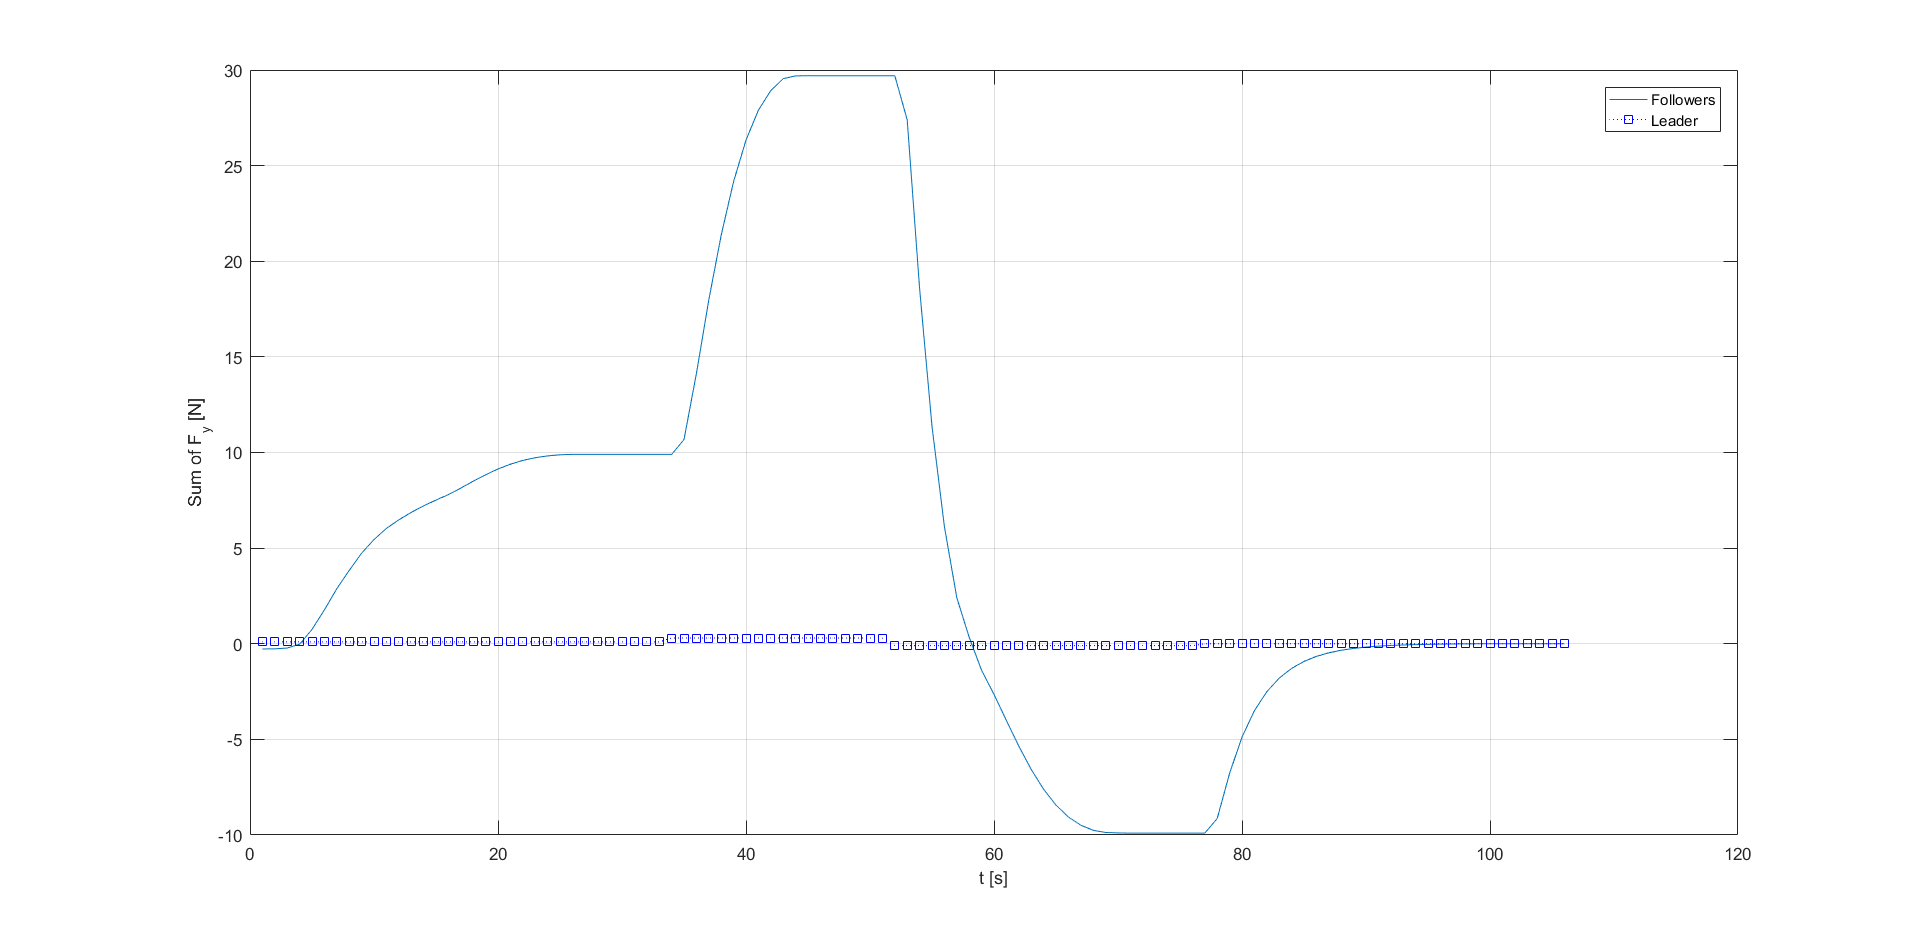
\includegraphics[width=.53\textwidth]{figures/P_ANTS_SumFy.png}
	\centering
	\caption{P-ANTS $\sum F_y$.}
	\label{fpsfy}
\end{figure}
\begin{figure}[!h]
	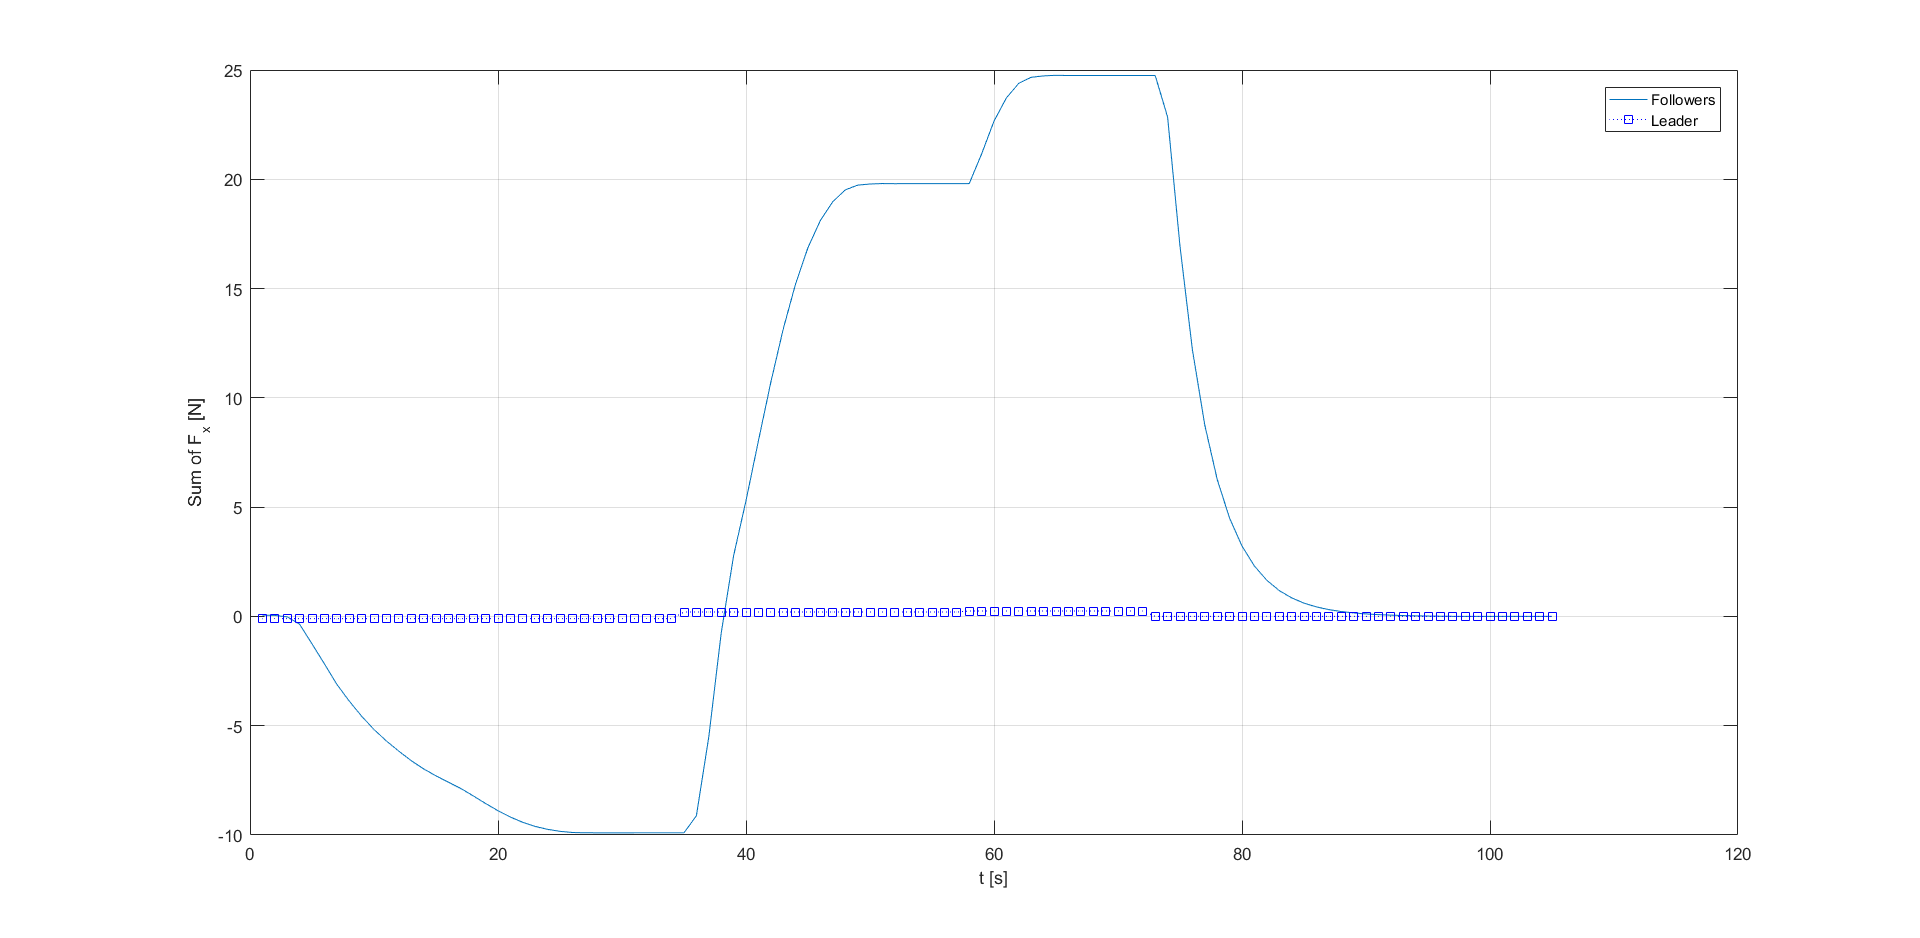
\includegraphics[width=.53\textwidth]{figures/P_ANTS_SumFx.png}
	\centering
	\caption{P-ANTS $\sum F_x$.}
	\label{fpsfx}
\end{figure}


%----------------------------------------------

\section{Conclusions}\label{concl}

\bibliographystyle{IEEEtrans}
\bibliography{IEEEabrv,mybib}

\end{document}